\documentclass[tikz]{standalone}
\date{}
\usepackage{amsmath,amsthm,amssymb}
\usepackage{xcolor}
\usepackage{tikz}
\usepackage[siunitx]{circuitikz}
\usepackage{tikz-3dplot}
\usepackage{ifthen}
\tikzset{isometricXYZ/.style={x={(-0.866cm,-0.5cm)}, y={(0.866cm,-0.5cm)}, z={(0cm,1cm)}}}
\usetikzlibrary{arrows,decorations.pathmorphing,positioning,fit,trees,shapes,automata,calc,intersections,decorations.markings,patterns,graphs,quotes,plotmarks}
%\usepackage{algorithm}
%\usepackage{algorithmic}
\newcommand{\R}{\mathbb{R}}
\newcommand{\F}{\mathbb{F}}
\newcommand{\bmat}[1]{\begin{bmatrix}#1\end{bmatrix}}
\newcommand{\xth}[1]{{#1}^{\mathrm{th}}}
\newcommand{\pd}[2]{\frac{\partial #1}{\partial #2} }
\newcommand{\pdd}[2]{\frac{\partial^2 #1}{\partial #2^2}}
\newcommand{\myitemsep}{\setlength\itemsep{-0.25em}}
\newcommand{\bigpar}[1]{\left( #1\right)}
\tikzset{myedge/.style={ thick,->,>=stealth',inner sep=0pt,outer sep=3pt}}
\tikzset{hv path/.style= {to path={-| (\tikztotarget)}}}
\tikzset{vh path/.style= {to path={|- (\tikztotarget)}}}

%%%%%%%%%% Using shift and rotate around:

\newcommand{\spring}[4]{
\path[shift={#1},rotate={#2},fill = white,opacity=1.0] (-0.25,-0.5) rectangle (0.25,0.5); % cover
\draw[thick,shift={#1},rotate={#2}] (0,0.5) -- +(0.25,-0.1) -- +(-0.25,-0.2)-- +(0.25,-0.3)-- +(-0.25,-0.4)-- +(0.25,-0.5)-- +(-0.25,-0.6)-- +(0.25,-0.7)-- +(-0.25,-0.8)-- +(0.25,-0.9) -- +(0,-1.0);
\draw[thick,shift={#1},rotate={#2}] (#3,0) node {#4};
}
\newcommand{\ground}[3]{
\draw[thick,shift={#1},rotate={#2}] (-0.5*#3cm,0) -- (0.5*#3cm,0);
\path[thick,shift={#1},rotate={#2},pattern=north west lines] (-0.5*#3cm,0) rectangle (0.5*#3cm,0.2);
}
\newcommand{\dashpot}[4]{
\path[shift={#1},rotate={#1},fill = white,opacity=1.0] (-0.25,0) rectangle (0.25,0.15);
\path[shift={#1},rotate={#1},draw,thick] (0,0) -- +(0.25,0) -- +(0.25,0.25) +(0.15,0.15) -- +(-0.15,0.15)  +(-0.25,0.25) -- +(-0.25,0) -- +(0,0);
\draw[thick,shift={#1},rotate={#1}] (#3,0) node {#4};
}
\newcommand{\mydashpot}[5]{
\begin{scope}[xshift=#1cm,yshift=#2cm,rotate=#3]
	\path[fill = white,opacity=1.0] (-0.25,0) rectangle (0.25,0.15);
	\path[draw,thick] (0,0) -- +(0.25,0) -- +(0.25,0.25) +(0.15,0.15) -- +(-0.15,0.15)  +(-0.25,0.25) -- +(-0.25,0) -- +(0,0);
	\node at (#4,0) {#5};
	\end{scope}
}
\newcommand{\lapof}[1]{\mathcal L \left\{ #1 \right\}}
\newcommand{\lapinv}[1]{\mathcal L^{-1} \left\{ #1 \right\}}
\newcommand{\evalat}[2]{\left. #1 \right|_{#2}}
\newcommand{\myarr}[3]{(-#2:#1) arc (-#2:#2:#1) node[#3] }
\newcommand{\mc}[1]{\mathcal{#1}}
\newcommand{\mred}[1]{\textcolor{red}{[#1]}}
\newcommand{\myco}[2]{\bigpar{ \frac{#1}{#2} }}
\newcommand{\tc}[2]{{#1}{#2}}
\newcommand{\mcb}[1]{{\color{blue}#1}}
\newcommand{\mcr}[1]{{\color{red}#1}}
\newcommand{\mcg}[1]{{\color{green!70!black}#1}}
\usepackage{hyperref}
\hypersetup{colorlinks=true,
linkcolor=blue,          % color of internal links
        citecolor=green,        % color of links to bibliography
          filecolor=magenta,      % color of file links
           urlcolor=blue           % color of external links
}

\usepackage{tkz-euclide}

\begin{document}

% \begin{tikzpicture}[every node/.style={scale=0.5}]
%     \coordinate [label=left:$P$] (P) at (0,0);
%     \coordinate [label=below:$Q$] (Q) at ($ (P) + 3/sqrt(5)*(2/3, -1/3) $);
%     \draw [name path=P--Q] (P) -- (Q);
% 
%     \coordinate [label=right:$R$] (R) at ($(Q) + (1, 1/2)$);
%     \draw [name path=Q--R] (Q) -- (R);
% 
%     \coordinate [label=above:$O$] (O) at ($(P) + 0.8*(1, 0.9)$);
%     \draw [name path=Q--R] (P) -- (O);
%     \draw [name path=O--Q] (O) -- (Q);
%     \draw [name path=O--R] (O) -- (R);
% 
%     \coordinate [label=below:$S$] (S) at ($ (P) + 3/sqrt(5)*(2/3, 1/3) $);
%     \draw[densely dashed] [name path=P--S] (P) -- (S);
%     \draw[densely dashed] [name path=S--R] (S) -- (R);
%     \draw[densely dashed] [name path=O--S] (O) -- (S);
% 
%     \node[label={[label distance=-1ex]30:$T$}] (T) at ($ (O)!0.5!(R) $) {};
%     \fill [red, opacity=0.5] (T) circle (1pt);
% \end{tikzpicture}

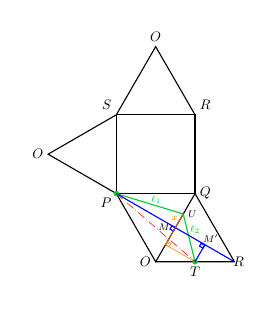
\begin{tikzpicture}[
    every node/.style={scale=0.5},
    ]
    \coordinate [label={[label distance=0ex]225:$P$}] (P) at (0,0);
    \coordinate [label={[label distance=0ex]0:$Q$}] (Q) at ($ (P) + (1,0) $);
    \coordinate [label={[label distance=0ex]45:$R$}] (R) at ($ (Q) + (0,1) $);
    \coordinate [label={[label distance=0ex]135:$S$}] (S) at ($ (P) + (0,1) $);
    \draw (P) -- (Q) -- (R) -- (S) -- (P);

    \coordinate (midPQ) at ($(P)!0.5!(Q)$);
    \coordinate [label={[label distance=0ex]180:$O$}] (O1) at ($(midPQ) +
        sqrt(3)/2*(0,-1)$);
    \draw (P) -- (O1) -- (Q);

    \coordinate [label={[label distance=-1ex]0:$R$}] (R1) at ($ (O1) + (1,0) $);
    \draw (O1) -- (R1) -- (Q);

    \coordinate (midPS) at ($(P)!0.5!(S)$);
    \coordinate [label={[label distance=0ex]180:$O$}] (O2) at ($(midPS) +
        sqrt(3)/2*(-1,0)$);
    \draw (P) -- (O2) -- (S);

    \coordinate (midSR) at ($(S)!0.5!(R)$);
    \coordinate [label={[label distance=0ex]90:$O$}] (O3) at ($(midSR) +
        sqrt(3)/2*(0,1)$);
    \draw (S) -- (O3) -- (R);

    \coordinate [label={[label distance=0ex]270:$T$}] (T) at ($ (O1)!0.5!(R1) $) {};
    \fill [green!80!blue, opacity=0.95] (T) circle (1pt);
    \fill [green!80!blue, opacity=0.95] (P) circle (1pt);

    \coordinate [label={[label distance=0ex]0:\scriptsize $U$}](btwOQ) at ($(O1)!0.7!(Q)$);
    \coordinate [label={[label distance=0.1ex]182:\scriptsize $M$}](midOQ) at ($(O1)!0.5!(Q)$);
    \draw[color=green!80!blue] (P) -- (btwOQ) -- (T);
    \draw[thin, color=blue] (P) -- (midOQ) -- (R1);

    \tkzMarkRightAngle[draw=blue, size=.05](P,midOQ,O1);

    \node [label={[label distance=-2ex]55:{\color{green!80!blue} \scriptsize $\ell_1$}}] (midPU) at ($ (P)!0.5!(btwOQ) $) {};
    \node [label={[label distance=-1.5ex]10:{\color{green!80!blue} \scriptsize $\ell_2$}}]
        (midUT) at ($ (btwOQ)!0.5!(T) $) {};
    \node [label={[label distance=-2ex]130:{\color{orange} \scriptsize $x$}}]
        (midMU) at ($ (midOQ)!0.5!(btwOQ) $) {};

    \coordinate [label={[label distance=-1.2ex]20:\scriptsize $M^\prime$}] (midMR) at ($ (midOQ)!0.5!(R1) $);
    \draw[color=blue] (T) -- (midMR);
    \tkzMarkRightAngle[draw=blue, size=.05](T,midMR,P);
    \tkzLabelAngle[dist=-0.035](T,midMR,P){$\color{blue} \cdot$};

    \coordinate [] (midOM) at ($ (O1)!0.5!(midOQ)$);
    \draw[very thin, color=orange] (T) -- (midOM) -- (btwOQ);
    \tkzMarkRightAngle[very thin, draw=orange, size=.05](T,midOM,btwOQ);
    \tkzLabelAngle[dist=0.035](T,midOM,btwOQ){$\color{orange} \cdot$};

    \draw[very thin, color=red, densely dashdotted] (P) -- (T);
\end{tikzpicture}

\end{document}
